\documentclass[12pt,a4paper]{article}

% ─── Page Layout ───────────────────────────────────────────────────────────────
\usepackage[a4paper, margin=0.8in, headheight=14pt]{geometry}

% ─── Fonts (XeLaTeX) ───────────────────────────────────────────────────────────
\usepackage{fontspec}
\usepackage{unicode-math}
\setmainfont{TeX Gyre Pagella}
\setmonofont[Scale=0.88]{TeX Gyre Cursor}
\setmathfont{Latin Modern Math}

% ─── Packages ──────────────────────────────────────────────────────────────────
\usepackage{xcolor}
\usepackage{colortbl}
\usepackage{titlesec}
\usepackage{enumitem}
\usepackage{tabularx}
\usepackage{booktabs}
\usepackage{array}
\usepackage{amsmath}
\usepackage{tikz}
\usetikzlibrary{shapes.geometric, arrows.meta, positioning, calc, fit, decorations.pathreplacing}
\usepackage{tcolorbox}
\tcbuselibrary{skins, breakable}
\usepackage{hyperref}
\usepackage{fancyhdr}
\usepackage{graphicx}
\usepackage{microtype}
\hyphenpenalty=10000
\exhyphenpenalty=10000
\sloppy
\usepackage{caption}
\usepackage{setspace}
\usepackage{multirow}
\usepackage{tocloft}

% ─── Q&A helper ────────────────────────────────────────────────────────────────
\newcommand{\Q}[1]{\textbf{#1}\par\noindent\ignorespaces}

% ─── Colour Palette ────────────────────────────────────────────────────────────
\definecolor{myred}{RGB}{196,30,58}
\definecolor{mydark}{RGB}{30,30,50}
\definecolor{mygreen}{RGB}{14,120,80}
\definecolor{myteal}{RGB}{0,130,140}
\definecolor{myamber}{RGB}{180,100,0}
\definecolor{mypurple}{RGB}{100,30,160}
\definecolor{mygray}{RGB}{246,247,249}
\definecolor{mgframe}{RGB}{180,185,200}
\definecolor{watermark}{RGB}{145,150,170}
\definecolor{hdrred}{RGB}{250,232,235}
\definecolor{hdrgreen}{RGB}{220,244,233}
\definecolor{hdrteal}{RGB}{220,242,244}
\definecolor{hdramber}{RGB}{253,242,215}
\definecolor{hdrpurple}{RGB}{238,228,255}
\definecolor{hdrgray}{RGB}{238,240,245}
\definecolor{rowalt}{RGB}{250,251,253}

% ─── Section Formatting ────────────────────────────────────────────────────────
\titleformat{\section}
  {\large\bfseries\color{myred}}{\thesection.}{0.5em}{}
  [\vspace{1pt}{\color{myred}\rule{\linewidth}{0.8pt}}]
\titleformat{\subsection}
  {\normalsize\bfseries\color{myteal}}{\thesubsection}{0.5em}{}
\titlespacing*{\section}{0pt}{18pt}{7pt}
\titlespacing*{\subsection}{0pt}{11pt}{4pt}

% ─── Paragraph ─────────────────────────────────────────────────────────────────
\setlength{\parindent}{0pt}
\setlength{\parskip}{4pt}

% ─── TOC Styling ───────────────────────────────────────────────────────────────
\renewcommand{\cfttoctitlefont}{\large\bfseries\color{myred}}
\renewcommand{\cftaftertoctitle}{\par\noindent{\color{myred}\rule{\linewidth}{0.8pt}}}
\setlength{\cftbeforetoctitleskip}{0pt}
\setlength{\cftaftertoctitleskip}{6pt}
\renewcommand{\cftsecfont}{\normalsize\bfseries\color{mydark}}
\renewcommand{\cftsecpagefont}{\normalsize\bfseries\color{mydark}}
\renewcommand{\cftsecleader}{\cftdotfill{\cftdotsep}}
\setlength{\cftbeforesecskip}{7pt}
\renewcommand{\cftsubsecfont}{\small\color{mydark}}
\renewcommand{\cftsubsecpagefont}{\small\color{mydark}}
\setlength{\cftbeforesubsecskip}{3pt}
\setlength{\cftsubsecindent}{1.4em}

% ─── Table helpers ─────────────────────────────────────────────────────────────
\renewcommand{\arraystretch}{1.45}
\setlength{\tabcolsep}{6pt}
\arrayrulecolor{mydark}
\newcolumntype{B}[1]{>{\small\bfseries\raggedright\arraybackslash}m{#1}}
\newcolumntype{Y}{>{\small\raggedright\arraybackslash}X}
\renewcommand{\tabularxcolumn}[1]{m{#1}}

% ─── Header / Footer ───────────────────────────────────────────────────────────
\pagestyle{fancy}
\fancyhf{}
\fancyhead[L]{\small\color{myred}\textbf{OE-EC704C}\;\color{mydark}--- Entrepreneurship}
\fancyhead[R]{\small\color{myteal}\textbf{Module 2 Notes}}
\fancyfoot[C]{\small\color{mydark}\thepage}
\fancyfoot[R]{\small\color{watermark}\textit{\copyright\ Biraj}}
\renewcommand{\headrulewidth}{0.5pt}
\renewcommand{\footrulewidth}{0.3pt}

% ─── Hyperref ──────────────────────────────────────────────────────────────────
\hypersetup{
  colorlinks=true, linkcolor=myteal, urlcolor=myteal,
  pdfauthor={Biraj Sarkar},
  pdftitle={OE-EC704C --- Module 2 Notes}
}

% ─── tcolorbox styles ──────────────────────────────────────────────────────────
\tcbset{
  tikzbox/.style={
    colback=mygray, colframe=mgframe, boxrule=0.6pt, arc=4pt,
    left=8pt, right=8pt, top=6pt, bottom=6pt,
    colbacktitle=mgframe, coltitle=mydark,
    fonttitle=\small\bfseries
  },
  defbox/.style={
    colback=hdrgreen, colframe=mygreen, boxrule=0.8pt, arc=4pt,
    left=9pt, right=9pt, top=6pt, bottom=6pt,
    colbacktitle=mygreen, coltitle=white,
    fonttitle=\small\bfseries
  },
  formulabox/.style={
    colback=hdrteal, colframe=myteal, boxrule=0.8pt, arc=4pt,
    left=9pt, right=9pt, top=7pt, bottom=7pt,
    colbacktitle=myteal, coltitle=white,
    fonttitle=\small\bfseries
  },
  examplebox/.style={
    colback=hdramber, colframe=myamber, boxrule=0.8pt, arc=4pt,
    left=9pt, right=9pt, top=6pt, bottom=6pt,
    colbacktitle=myamber, coltitle=white,
    fonttitle=\small\bfseries
  },
  masonbox/.style={
    colback=hdrpurple, colframe=mypurple, boxrule=0.8pt, arc=4pt,
    left=9pt, right=9pt, top=6pt, bottom=6pt,
    colbacktitle=mypurple, coltitle=white,
    fonttitle=\small\bfseries
  },
  exambox/.style={
    colback=hdrpurple, colframe=mypurple, boxrule=1pt, arc=5pt,
    left=10pt, right=10pt, top=8pt, bottom=8pt,
    colbacktitle=mypurple, coltitle=white,
    fonttitle=\bfseries,
    breakable, title after break={\textbf{Frequently Asked / Viva Questions (contd.)}}}
}
\tcbset{breakable}

% ─── TikZ styles ───────────────────────────────────────────────────────────────
\tikzset{
  block/.style={rectangle, draw=myteal, fill=hdrteal,
    text width=2.4cm, align=center, minimum height=0.95cm,
    font=\small, rounded corners=3pt, line width=0.7pt},
  redblock/.style={rectangle, draw=myred, fill=hdrred,
    text width=2.4cm, align=center, minimum height=0.95cm,
    font=\small, rounded corners=3pt, line width=0.7pt},
  netnode/.style={rectangle, draw=myteal, fill=hdrteal,
    text width=1.5cm, align=center, minimum height=0.8cm,
    font=\small, rounded corners=3pt, line width=0.7pt},
  sumjunc/.style={circle, draw=myamber, fill=hdramber,
    minimum size=0.62cm, font=\small, line width=0.8pt},
  snode/.style={circle, draw=mypurple, fill=hdrpurple,
    minimum size=0.55cm, font=\footnotesize, line width=0.7pt},
  arrow/.style={-Stealth, thick, color=mydark},
  redarrow/.style={-Stealth, thick, color=myred},
  line/.style={thick, color=mydark}
}

% ═══════════════════════════════════════════════════════════════════════════════
\begin{document}
% ═══════════════════════════════════════════════════════════════════════════════

\begin{center}
  {\LARGE\bfseries\color{myred} OE-EC704C --- Entrepreneurship}\\[5pt]
  {\normalsize\color{mydark} Semester VII \quad$\bullet$\quad 3L:0T:0P \quad$\bullet$\quad 3 Credits}\\[3pt]
  {\normalsize\color{myteal}\textbf{Module 2 Exam Notes: Marketing, Financing \& Launching}}\\[3pt]
  {\small\color{mydark} CGEC \;$|$\; B.Tech ECE (2023--27) \;$|$\; \textit{Biraj Sarkar}}
\end{center}
\vspace{2pt}
\noindent{\color{myred}\rule{\linewidth}{1.5pt}}
\vspace{2pt}

\hypersetup{linkcolor=mydark}
\tableofcontents
\hypersetup{linkcolor=myteal}
\newpage

% ===============================================================================
\section{Market Survey and Research}
% ===============================================================================

Before launching any product, an entrepreneur must understand consumer needs, market demand, and competitor behaviors. This is achieved through systematic market research and surveys.

\subsection{Market Survey vs. Market Research}
\begin{itemize}[leftmargin=*, itemsep=3pt]
  \item \textbf{Market Research:} A broad, systematic process of collecting, analyzing, and interpreting data about a market, including its size, segmentation, trends, competitors, and regulatory environment.
  \item \textbf{Market Survey:} A specific quantitative tool used within market research to gather structured opinions, feedback, or demographics from a representative sample of potential customers.
\end{itemize}

\subsection{Data Collection Methodologies}
\par\noindent
{\renewcommand{\arraystretch}{1.5}%
\begin{tabularx}{\linewidth}{|B{3.0cm}|Y|Y|}\hline
\multicolumn{1}{|>{\centering\arraybackslash}m{3.0cm}|}{\textbf{Feature}} &
\multicolumn{1}{>{\centering\arraybackslash}Y|}{\textbf{Primary Data}} &
\multicolumn{1}{>{\centering\arraybackslash}Y|}{\textbf{Secondary Data}} \\
\hline
\textbf{Definition} & Firsthand data collected directly for the specific research purpose. & Existing data gathered by third parties for other purposes. \\
\hline
\textbf{Methods} & Questionnaires, direct interviews, focus groups, observations. & Government census reports, industry journals, trade databases. \\
\hline
\textbf{Cost \& Time} & Highly expensive and time-consuming. & Relatively inexpensive and instantly accessible. \\
\hline
\textbf{Relevance} & 100\% tailored to the entrepreneur's immediate needs. & May be outdated, generic, or not fully aligned. \\
\hline
\textbf{Accuracy} & Controlled directly; high reliability. & Variable quality; requires validation. \\
\hline
\end{tabularx}
}

\subsection{Product Pricing Techniques}
Pricing directly determines sales velocity and profit margins. Entrepreneurs use several strategic pricing techniques:
\begin{enumerate}[label=\textbf{\arabic*.}, leftmargin=*, itemsep=4pt]
  \item \textbf{Cost-Plus Pricing (Markup Pricing):} The simplest method. A fixed percentage profit margin (markup) is added to the total cost of producing the product.
    \begin{equation}
      \text{Price} = \text{Unit Cost} \times (1 + \text{Markup Percentage})
    \end{equation}
  \item \textbf{Penetration Pricing:} Setting a very low initial price to attract a large volume of buyers quickly, establish market share, and discourage competitors. Prices are raised later once customer loyalty is secured.
  \item \textbf{Skimming Pricing:} Setting a high price initially for a new, innovative, or premium product to capture the maximum revenue from early adopters (who are less price-sensitive). Prices are lowered gradually to target broader segments.
  \item \textbf{Competitive Pricing:} Aligning the price directly with the prevailing market rates of close competitors, adjusting slightly for brand differentiation.
  \item \textbf{Demand-Based Pricing (Value-Based Pricing):} Setting prices primarily based on the perceived value to the consumer rather than the production cost (e.g., dynamic airline ticket pricing, premium software).
\end{enumerate}

% ===============================================================================
\section{Distribution Channels and Sales Promotion}
% ===============================================================================

\subsection{Distribution Channels}
\begin{tcolorbox}[defbox, title={Definition of Distribution Channel}]
A \textbf{Distribution Channel} (or marketing channel) is the pathway or chain of intermediaries (such as wholesalers, retailers, and agents) through which a product travels from the point of manufacture to the final consumer.
\end{tcolorbox}

\subsubsection{Types of Distribution Channels}
Distribution channels are classified based on the number of intermediary levels involved:

\begin{tcolorbox}[tikzbox, title={Structure of Distribution Channels}]
\centering
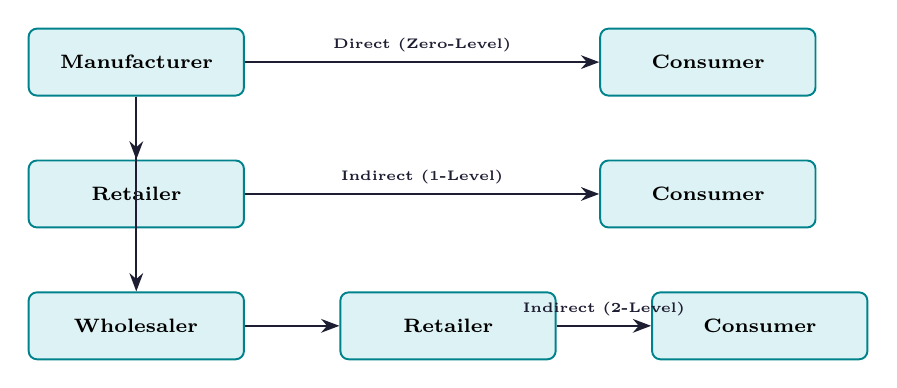
\begin{tikzpicture}[
  node distance=0.8cm and 1.2cm,
  block/.style={rectangle, draw=myteal, fill=hdrteal, text width=2.5cm, align=center, minimum height=0.85cm, font=\scriptsize\bfseries, rounded corners=3pt, line width=0.7pt},
  arrow/.style={-Stealth, thick, color=mydark}
]
  \node[block] (m) {Manufacturer};
  
  % Level 0
  \node[block, right=4.5cm of m] (c1) {Consumer};
  \draw[arrow] (m) -- node[above, font=\tiny\bfseries\color{myred}] {Direct (Zero-Level)} (c1);
  
  % Level 1
  \node[block, below=of m] (r) {Retailer};
  \node[block, right=4.5cm of r] (c2) {Consumer};
  \draw[arrow] (m) -- (r);
  \draw[arrow] (r) -- node[above, font=\tiny\bfseries\color{myteal}] {Indirect (1-Level)} (c2);
  
  % Level 2
  \node[block, below=of r] (w) {Wholesaler};
  \node[block, right=of w] (r2) {Retailer};
  \node[block, right=of r2] (c3) {Consumer};
  \draw[arrow] (m) -- (w);
  \draw[arrow] (w) -- (r2);
  \draw[arrow] (r2) -- node[above, font=\tiny\bfseries\color{myamber}] {Indirect (2-Level)} (c3);
\end{tikzpicture}
\end{tcolorbox}

\subsubsection{Factors Influencing Channel Selection}
An entrepreneur must select channels based on four critical factors:
\begin{itemize}[leftmargin=*, itemsep=3pt]
  \item \textbf{Product Characteristics:} Perishable goods (e.g., food) require direct/short channels. Industrial, high-value, or customized items (e.g., machinery) also use direct sales, while standardized, durable consumer goods use multi-level channels.
  \item \textbf{Market Factors:} A scattered consumer base requires wholesalers and retailers. If the target market is small and concentrated, direct selling is optimal.
  \item \textbf{Company Resources:} Startups with limited capital and sales force rely on existing distributor networks. Strong companies can establish direct retail outlets.
  \item \textbf{Middlemen Capability:} Availability of reliable distributors, credit-worthiness, and the margin share they demand.
\end{itemize}

\subsection{Sales Promotion Activities}
Sales promotion includes short-term incentives to encourage quick purchases of a product.
\begin{itemize}[leftmargin=*, itemsep=3.5pt]
  \item \textbf{Consumer-Oriented Promotions:} Target the end customer directly.
    \begin{itemize}[label=\tiny$\bullet$, leftmargin=1.5em, itemsep=2pt]
      \item \textit{Price Discounts \& Rebates:} Temporary price cuts (e.g., 20\% off, ``Buy 1 Get 1 Free'').
      \item \textit{Coupons:} Certificates offering a specified discount on purchase.
      \item \textit{Free Samples:} Distributing small quantities of the product to encourage trial.
      \item \textit{Contests/Sweepstakes:} Competitions where buyers stand a chance to win prizes.
    \end{itemize}
  \item \textbf{Trade-Oriented Promotions:} Target intermediaries (distributors, retailers) to push the product.
    \begin{itemize}[label=\tiny$\bullet$, leftmargin=1.5em, itemsep=2pt]
      \item \textit{Trade Allowances:} Financial incentives/discounts for stocking and displaying products.
      \item \textit{Cooperative Advertising:} Manufacturer shares local advertising costs with the retailer.
      \item \textit{Dealer Sales Contests:} Rewarding dealers who achieve peak sales volumes.
    \end{itemize}
\end{itemize}

% ===============================================================================
\section{Raising Business Finance}
% ===============================================================================

Capital is the lifeblood of any enterprise. Financing is categorized into Equity (ownership capital) and Debt (borrowed capital).

\subsection{Debt vs. Equity Financing}
\par\noindent
{\renewcommand{\arraystretch}{1.5}%
\begin{tabularx}{\linewidth}{|B{2.8cm}|Y|Y|}\hline
\multicolumn{1}{|>{\centering\arraybackslash}m{2.8cm}|}{\textbf{Parameter}} &
\multicolumn{1}{>{\centering\arraybackslash}Y|}{\textbf{Equity Financing}} &
\multicolumn{1}{>{\centering\arraybackslash}Y|}{\textbf{Debt Financing}} \\
\hline
\textbf{Ownership} & Dilutes ownership; investors get voting rights and shares. & No dilution of ownership; lender has no say in management. \\
\hline
\textbf{Repayment} & No obligation to repay; profits are distributed as dividends. & Legal obligation to make regular principal and interest payments. \\
\hline
\textbf{Collateral} & No collateral or asset pledge required. & Often requires tangible assets or personal guarantees. \\
\hline
\textbf{Cost} & High cost in the long run (giving away future profits). & Lower cost (fixed interest rate, which is tax-deductible). \\
\hline
\textbf{Risk} & Zero bankruptcy risk; safe for early-stage ventures. & High risk; default can lead to asset foreclosure and insolvency. \\
\hline
\end{tabularx}
}

\subsection{Sources of Startup Finance}
\begin{enumerate}[label=\textbf{\arabic*.}, leftmargin=*, itemsep=4pt]
  \item \textbf{Bootstrapping (Self-Funding):} The entrepreneur uses personal savings, credit cards, or loans from friends/family. It retains 100\% equity but limits growth scope.
  \item \textbf{Angel Investors:} Wealthy individuals who invest their personal capital in early-stage startups in exchange for equity. They also provide mentorship and networks.
  \item \textbf{Venture Capital (VC):} Professional firms that manage pooled funds from institutional investors to invest in high-growth, scalable startups. They invest larger tickets during Series A, B, etc., and demand board seats.
  \item \textbf{Commercial Banks \& Financial Institutions:} Conventional term loans or lines of credit. Suitable for asset acquisition (machinery/land) once the business has cash flow.
  \item \textbf{Government Initiatives (India):}
    \begin{itemize}[label=\tiny$\bullet$, leftmargin=1.5em, itemsep=2pt]
      \item \textit{MUDRA Loans (PMMY):} Low-interest loans up to $\text{Rs. } 10 \text{ Lakhs}$ under Shishu, Kishor, and Tarun schemes for micro-enterprises.
      \item \textit{Startup India Seed Fund Scheme (SISFS):} Provides grants/loans to startups for proof of concept, prototype development, and market entry.
    \end{itemize}
\end{enumerate}

% ===============================================================================
\section{Enterprise Launching Formalities}
% ===============================================================================

Once the finance is secured and the product is finalized, the entrepreneur must complete the legal launching process:

\subsection{Legal Formality Checklist}
\begin{itemize}[leftmargin=*, itemsep=3.5pt]
  \item \textbf{Entity Registration:} Register the business name and structure (Ministry of Corporate Affairs for Private Ltd/LLP, or local Registrar of Firms for Partnership).
  \item \textbf{Tax Registrations:}
    \begin{itemize}[label=\tiny$\bullet$, leftmargin=1.5em, itemsep=2.0pt]
      \item \textit{Permanent Account Number (PAN):} Required for all corporate banking and tax filings.
      \item \textit{GSTIN Registration:} Mandatory for businesses with inter-state sales or annual turnover exceeding the threshold ($\text{Rs. } 40 \text{ Lakhs}$ for goods / $\text{Rs. } 20 \text{ Lakhs}$ for services).
    \end{itemize}
  \item \textbf{Municipal/Local Licenses:} Trade License from the local Municipal Corporation, and Shops and Establishment Act registration.
  \item \textbf{Environmental and Safety Approvals:} Consent to Establish (CTE) and Consent to Operate (CTO) from the State Pollution Control Board (SPCB) for manufacturing units. Fire safety clearance.
  \item \textbf{Udyam (MSME) Registration:} Completed online for benefits under government procurement and priority lending schemes.
  \item \textbf{Commercial Bank Account:} Opening a current account in the name of the registered entity to keep business transactions separate.
\end{itemize}

\newpage

% ===============================================================================
% MANDATORY QUICK REVISION PAGE
% ===============================================================================
\begin{center}
  {\large\bfseries\color{myred} Quick Revision --- Module 2}\\[3pt]
  {\small\color{mydark} Marketing, Financing \& Launching $|$ OE-EC704C}
\end{center}
\noindent{\color{myred}\rule{\linewidth}{1.2pt}}
\vspace{4pt}

\begin{tcolorbox}[formulabox, title={\textbf{Key Concepts at a Glance}}]
\renewcommand{\arraystretch}{1.3}
\begin{tabularx}{\linewidth}{B{4.0cm} X}
Primary Data & Firsthand market feedback (custom, expensive, accurate). \\
Skimming Pricing & High initial price for innovative products $\rightarrow$ lower gradually. \\
Penetration Pricing & Low initial price to capture market share $\rightarrow$ raise later. \\
Markup Formula & $\text{Selling Price} = \text{Unit Cost} \times (1 + \text{Markup \%})$. \\
Zero-Level Channel & Direct path: $\text{Manufacturer} \rightarrow \text{Consumer}$ (no middlemen). \\
Angel Investors & Wealthy individuals investing personal money in early-stage startups. \\
GSTIN & 15-digit unique Goods and Services Tax Identification Number. \\
\end{tabularx}
\end{tcolorbox}

\begin{tcolorbox}[defbox, title={\textbf{One-Line Definitions}}]
\begin{itemize}[leftmargin=*, itemsep=2.5pt, topsep=0pt]
  \item \textbf{Market Research:} Systematic process of gathering and analyzing data about a target market and its competitors.
  \item \textbf{Value-Based Pricing:} Setting price based on the customer's perceived value rather than production cost.
  \item \textbf{Distribution Channel:} Chain of businesses or intermediaries through which a product passes to the final buyer.
  \item \textbf{Sales Promotion:} Short-term incentives designed to stimulate immediate demand and sales.
  \item \textbf{Equity Financing:} Raising capital by selling shares of ownership in the company.
  \item \textbf{Debt Financing:} Borrowing capital that must be repaid over time with interest.
  \item \textbf{Venture Capital:} Funds invested in high-risk, high-growth startups by professional firms.
\end{itemize}
\end{tcolorbox}

\begin{tcolorbox}[exambox, title={\textbf{Frequently Asked / Viva Questions}}]
\begin{enumerate}[topsep=0pt, label=\textbf{Q\arabic*.}, itemsep=5pt]
  \item \Q{Compare primary data and secondary data in market surveys.}
    Primary data is collected firsthand for the specific study (e.g., questionnaires) and is highly relevant but expensive. Secondary data already exists (e.g., government reports) and is cheap and fast but might be generic or outdated.
  \item \Q{When is Skimming Pricing used instead of Penetration Pricing?}
    Skimming is used for highly innovative, patented, or luxury products to recover development costs from early adopters. Penetration is used in highly competitive markets to capture rapid volume and build a barrier for rivals.
  \item \Q{What is a Zero-Level distribution channel? Give an example.}
    It is a direct channel where the manufacturer sells directly to the consumer without any intermediaries. Examples: factory outlets, e-commerce websites, and door-to-door sales.
  \item \Q{What factors dictate the selection of a distribution channel?}
    Product characteristics (perishability, value), market characteristics (customer density, geography), company resources (budget, sales force), and middlemen capabilities (margins, reach).
  \item \Q{Differentiate between consumer promotion and trade promotion.}
    Consumer promotion targets the end-user (e.g., coupons, free samples) to pull products off shelves. Trade promotion targets wholesalers/retailers (e.g., display allowances, trade discounts) to push products through the channel.
  \item \Q{Why is debt financing considered cheaper than equity financing in the long run?}
    Interest payments on debt are fixed and tax-deductible, and debt does not dilute ownership or future profits. Equity dilute ownership permanently, making it expensive if the company grows highly profitable.
  \item \Q{Define Venture Capital (VC).}
    Venture Capital is professional private equity investment provided to early-stage, high-potential startups with high growth scalability, in exchange for equity and significant managerial influence.
  \item \Q{What is the purpose of Udyam registration for a launching startup?}
    It provides MSME classification, which unlocks interest rate concessions on bank loans, collateral-free credit guarantees, subsidies on patents, and eligibility for government procurement tenders.
  \item \Q{What are the mandatory tax registrations required to start commercial sales in India?}
    Permanent Account Number (PAN) for income tax and financial transactions, and Goods and Services Tax Identification Number (GSTIN) for indirect tax compliance.
  \item \Q{Name two government financing schemes for MSMEs in India.}
    The MUDRA Yojana (PMMY) for micro-loans up to $\text{Rs. } 10 \text{ Lakhs}$, and the Startup India Seed Fund Scheme (SISFS) for early-stage proof-of-concept capital.
  \end{enumerate}
\end{tcolorbox}

\end{document}
